\section{単純支持されたプレートの圧縮時の座屈}
この例では、単純支持された長方形のプレートのすべての端が圧縮された場合の座屈を解析します。
その寸法は:
\begin{itemize}
\item プレートサイズ:200$\times$150mm
\end{itemize}
ジオメトリーは、CADソフトウェアでサーフェスとしてモデリングされています。
\begin{enumerate}
\item
	{[}mm, ton, s, °C{]}単位の新規ファイルを作成し、ステップ形式のジオメトリをPrePoMaxにインポートします。
	次に、パーツをメッシュ分割します。
	ここでは、最大要素サイズとして5mmを選択し、四分割メッシュを有効にして、その他の設定は変更しませんでした(図\ref{fig:10-01})。
	\begin{figure}[H]
	\centering
	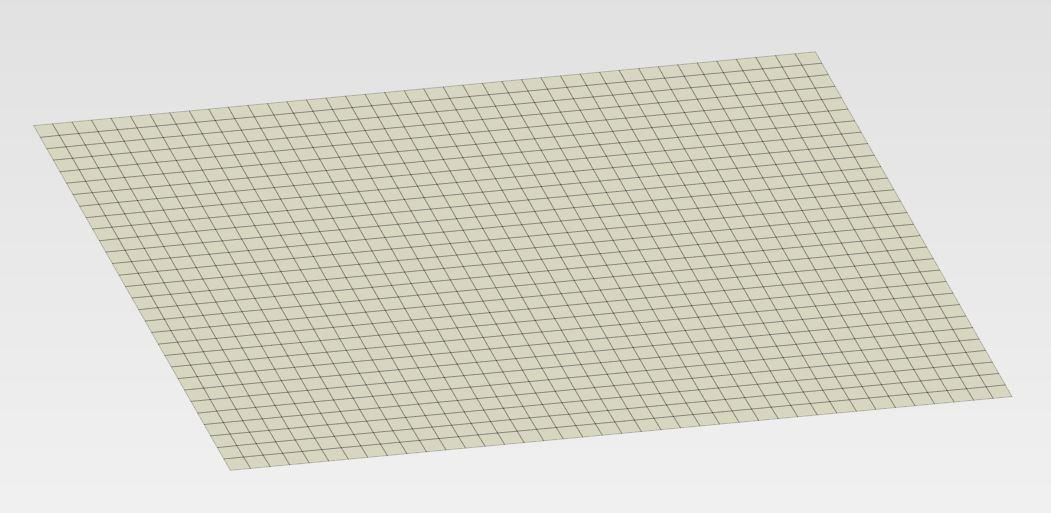
\includegraphics[width=133mm]{fig/10-01.png}
	\caption{プレート - メッシュ}
	\label{fig:10-01}
	\end{figure}
	\vspace{-\baselineskip}
\item
  新しい材料を定義し、弾性挙動を加え、ヤング率を200000MPa、ポアソン比を0.3と指定します。
  先に作成した材料を参照して新しいシェルセクションを作成し、そのセクションがこのパーツに割り当てられるようにプレートを選択します。
  厚さを4mmに指定します。
\item
  新しい座屈ステップを追加し、座屈係数の数を3に設定します。
  プレートのすべてのエッジに割り当てられた変位/回転境界条件を作成し、面外方向の移動のみを拘束します。
  さらに2つの変位/回転境界条件を追加して、プレートの垂直な2つのエッジに適用し、各エッジの法線方向を拘束する。
  法線方向のシェルエッジ荷重を1N/mmの大きさで定義し、法線方向のBCを持つエッジと反対側の2つのエッジに割り当てます(図\ref{fig:10-02})。
	\begin{figure}[H]
	\centering
	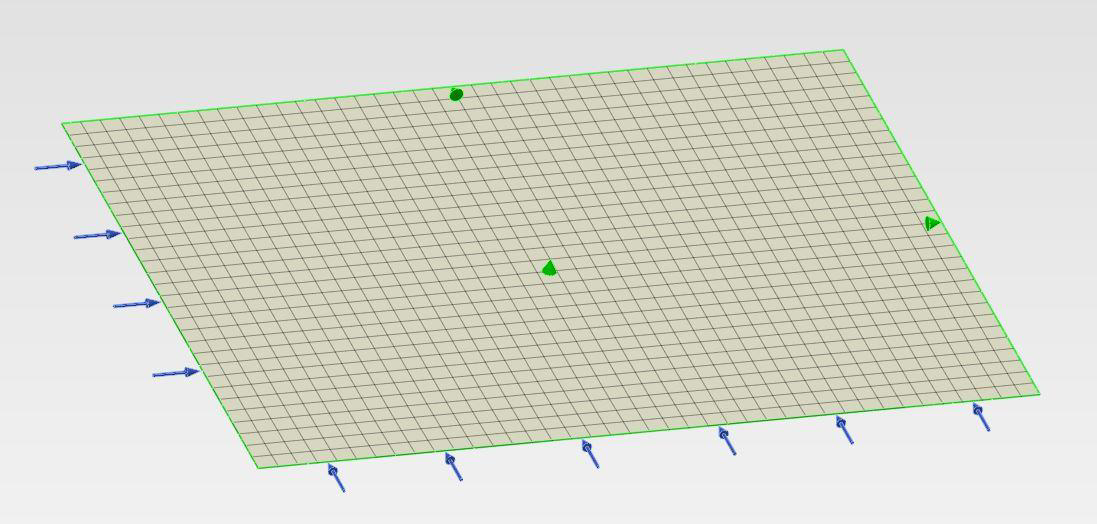
\includegraphics[width=137mm]{fig/10-02.png}
	\caption{プレート - 境界条件と荷重}
	\label{fig:10-02}
	\end{figure}
	\vspace{-\baselineskip}
\item
  解析を実行し、解析が終了したら結果を確認します。
  各座屈モード形状を確認します。2つ目は、下の画像のようになります(図\ref{fig:10-03})。
  分析的に計算した限界圧縮応力は200.85MPaですが、シミュレーションでは197MPaとなります。
	\begin{figure}[H]
	\centering
	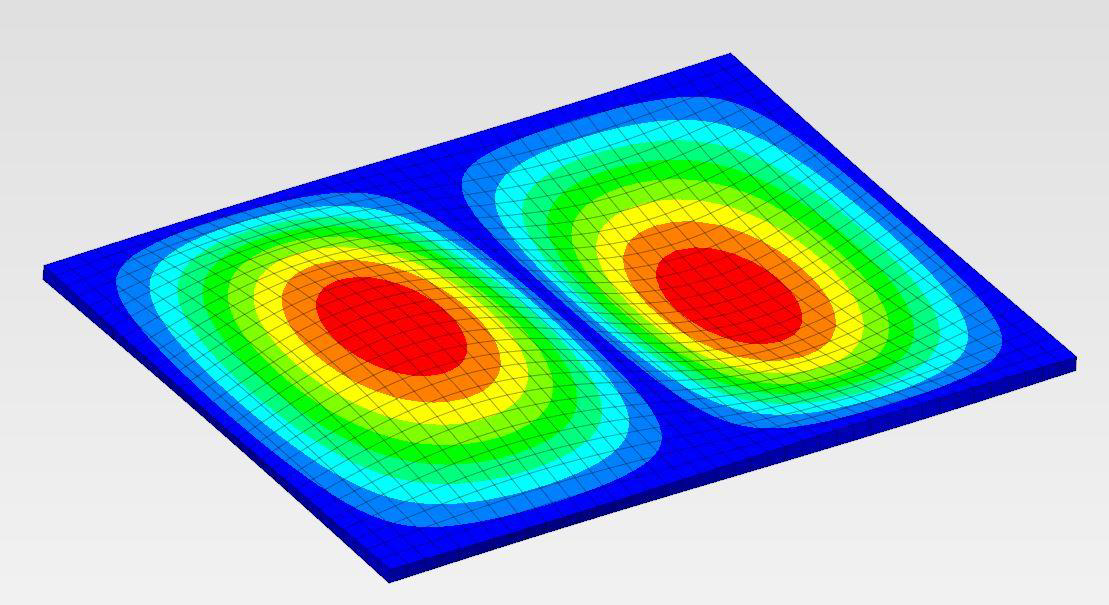
\includegraphics[width=138mm]{fig/10-03.png}
	\caption{プレート - 座屈モード形状 \#2}
	\label{fig:10-03}
	\end{figure}
\end{enumerate}